\documentclass[aspectratio=169]{beamer}
\usepackage{graphicx}
\usepackage{circuitikz}
\usepackage{tikz}
\usepackage{subcaption}
\graphicspath{ {../images/} }
\usetheme{Hannover}

\title{PDI: Control of a Soft Elbow Orthosis}
\author{David Kirov}
\date{\today}

\begin{document}

\begin{frame}
\titlepage
\end{frame}

\begin{frame}{Outline}
\tableofcontents
\end{frame}

\section{Introduction}
\begin{frame}{Introduction}
\begin{columns}
\begin{column}{0.6\textwidth}
What are orthoses?  

\bigskip 

Active/passive orthoses.  

\bigskip

Why are active orthotic devices needed?  
\begin{itemize}
  \item Loss of motor function
  \item Rehabilitation for neuroplasticity
\end{itemize}

\bigskip

Objectives

\end{column}
\begin{column}{0.4\textwidth}
\begin{figure}[htbp]
  \centering
  \includegraphics[width=0.6\linewidth]{passive_orthosis.jpg}
  \caption{Ankle-foot passive orthosis}
  \label{fig:passive_orthosis}
\end{figure}
\end{column}
\end{columns}
\end{frame}

\section{SysML Models}
\begin{frame}{SysML Models}
\begin{figure}[htbp]
  \centering
  \includegraphics[width=0.6\textwidth]{context.png}
  \caption{Context diagram}
  \label{fig:context_diagram}
\end{figure}
\end{frame}
\begin{frame}{SysML Models}
\begin{figure}[htbp]
  \centering
  \includegraphics[width=\textwidth]{use_case.png}
  \caption{Use case diagram}
  \label{fig:use_case_diagram}
\end{figure}
\end{frame}
\begin{frame}{SysML Models}
\begin{figure}[htbp]
  \centering
  \includegraphics[width=\textwidth]{requirement.png}
  \caption{Requirement table}
  \label{fig:requirements_table}
\end{figure}
\end{frame}

\section{Materials and methods}
\subsection{Hardware}
\begin{frame}{Hardware}
\begin{itemize}
  \item Sensor system 
  \item Maxon 150W BLDC motor
  \item Maxon EPOS4 driver
  \item 64bit Linux PC (Fedora 39)
  \item 3A - 30V power supply
\end{itemize}
\begin{figure}
    \centering
    \begin{subfigure}{0.2\textwidth}
        \centering
        \includegraphics[width=\linewidth]{myoware_sensor.jpg}
        \caption{Myoware muscle sensor}
        \label{fig:myoware_sensor}
    \end{subfigure}
    \begin{subfigure}{0.14\textwidth}
        \centering
        \includegraphics[width=\linewidth]{bno055_sensor.jpg}
        \caption{BNO055}
        \label{fig:bno_sensor}
    \end{subfigure}
    \begin{subfigure}{0.27\textwidth}
        \centering
        \includegraphics[width=\linewidth]{esp32.jpg}
        \caption{ESP32}
        \label{fig:esp32}
    \end{subfigure}
    \caption{
      Sensors and microcontroller
    }
    \label{fig:sensor_system}
\end{figure}
\end{frame}

\subsection{Communication Strategy}
\begin{frame}{Communication Strategy}
\centering
\resizebox{\linewidth}{!}{%
	\begin{circuitikz}[auto,>=latex]
	    \node[draw, rectangle] (MC) at (0,0) {ESP32};
	    \node[draw, rectangle] (PC) at (3,0) {PC};
	    \node[draw, rectangle] (EPOS4) at (7,0) {
		  \begin{tabular}{c}
		    EPOS4\\ 
		    Driver
		  \end{tabular}
		};
	    \node[draw, rectangle] (Motor) at (10,0) {Motor};
	    \node[draw, rectangle] (IMU1) at (0,2) {IMU 1};
	    \node[draw, rectangle] (IMU2) at (-3,2) {IMU 2};
	    \node[draw, rectangle] (Myo) at (-3,0) {Myo};
	    \draw [->] (IMU1) -- (MC) node[midway,right] {I2C};
	    \draw (IMU1) -- (IMU2) node[midway,above] {I2C};
	    \draw [->] (Myo) -- (MC) node[midway,above] {Analog};
	    \draw [->] (MC) -- (PC) node[midway,above] {BLE};
	    \draw [<->] (PC) -- (EPOS4) node[midway,above] {Serial};
	    \draw (EPOS4) -- (Motor) node[midway,above] {};
	\end{circuitikz}
}
\end{frame}

\subsection{Control Strategy}
\begin{frame}{Control Strategy}
\centering
\resizebox{\linewidth}{!}{%
	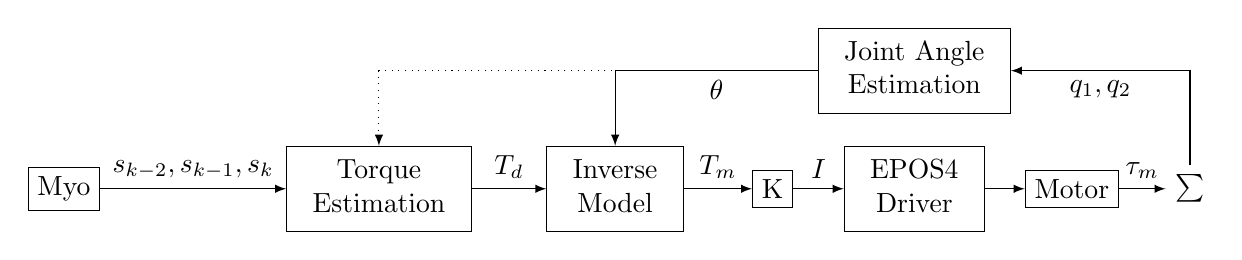
\begin{tikzpicture}[auto, >=latex]
	\tikzstyle{block} = [draw, rectangle]

	\node [block, draw] (input) at (0,0) {Myo};
	\node [block, draw, right of=input, node distance=4cm] (alg) {%
	  \begin{tabular}{c}
	    Torque\\ 
	    Estimation
	  \end{tabular}
	};
	\node [block, right of=alg, node distance=3cm] (inv-model) {
	  \begin{tabular}{c}
	    Inverse\\ 
	    Model
	  \end{tabular}
	};
	\node [block, right of=inv-model, node distance=2cm] (gain) {K};
	\node [block, right of=gain, node distance=1.8cm] (driver) {
	  \begin{tabular}{c}
	    EPOS4\\ 
	    Driver
	  \end{tabular}
	};
	\node [block, above of=driver, node distance=1.5cm] (angle) {
	  \begin{tabular}{c}
	    Joint Angle\\ 
	    Estimation
	  \end{tabular}
	};
	\node [block, right of=driver, node distance=2cm] (motor) {Motor};
	\node [right of=motor, node distance=1.5cm] (sys) {$\sum$};

	\draw [->] (input) -- node[above] {$s_{k-2},s_{k-1},s_k$} (alg);
	\draw [->] (alg) -- node[above] {$T_d$} (inv-model);
	\draw [->] (inv-model) -- node[above] {$T_m$} (gain);
	\draw [->] (gain) -- node[above] {$I$} (driver);
	\draw [->] (driver) -- (motor);
	\draw [->] (motor) -- node[above] {$\tau_m$} (sys);
	\draw [->] (sys) |- node[near end] {$q_1,q_2$} (angle);
	\draw [->] (angle) -| node[near start] {$\theta$} (inv-model);
	\draw [->, dotted] (angle) -| (alg);
	\end{tikzpicture}
}
\end{frame}

\subsection{Torque estimation}
\begin{frame}{Torque estimation}
Single-layer sequential neural network.  

\bigskip

Single and multi-dataset models were trained.  

4 models in total, differing in inputs:
\begin{itemize}
  \item open: $(s_{k-2},s_{k-1},s_k)$
  \item closed: $(s_{k-2},s_{k-1},s_k,\theta)$
\end{itemize}
\end{frame}
\begin{frame}{Torque estimation}
	Training data (sEMG, $\theta$) gathered at INRIA.

	\begin{columns}
	\begin{column}{0.5\textwidth}

	\begin{figure}[htbp]
	  \centering
	  \includegraphics[width=\linewidth]{processing.png}
	  \caption{Signal processing}
	  \label{fig:processing}
	\end{figure}
	\end{column}
	\begin{column}{0.4\textwidth}
	\begin{figure}[htbp]
	  \centering
	  \includegraphics[width=\linewidth]{processed.png}
	  \caption{Processed signal}
	  \label{fig:processed}
	\end{figure}
	\end{column}
	\end{columns}
\end{frame}

\begin{frame}{Torque estimation}
Torque calculation from angle measurement:
\begin{equation}
  \centering
  \tau=((m+\omega)l_{cm}^2+J)\ddot{\theta}+\beta \dot{\theta}+(ml_{cm}+\omega l)g\sin{\theta}
  \label{eq:torque}
\end{equation}
\begin{itemize}
  \item $m$ mass of the subject forearm and arm
  \item $\omega$ mass of the carried load
  \item $l$ distance from the elbow to the center of the hand
  \item $l_{cm}$ is the distance from the elbow to the forearm center of mass
  \item $J$ moment of inertia of the forearm
  \item $g$ gravitational acceleration 
  \item $\beta$ joint friction
\end{itemize}
\end{frame}

\begin{frame}{Torque estimation}
\begin{figure}[htbp]
  \centering
  \includegraphics[width=0.8\linewidth]{torque_from_angle.png}
  \caption{Torque and angle relationship}
  \label{fig:torque_from_angle}
\end{figure}
\end{frame}

\subsection{Orthosis model}
\begin{frame}{Orthosis model}
\begin{figure}[htbp]
\begin{columns}
\begin{column}{0.5\textwidth}
    \centering
    \begin{subfigure}{0.2\textwidth}
        \centering
        \includegraphics[width=\linewidth]{elbow.png}
        \caption{Elbow model}
        \label{fig:elbow}
    \end{subfigure}
    \begin{subfigure}{0.3\textwidth}
        \centering
        \includegraphics[width=\linewidth]{motor_torque.png}
        \caption{Motor front view}
        \label{fig:motor}
    \end{subfigure}
    \caption{
      Simplified orthosis model
    }
    \label{fig:orthosis_model}
    \end{column}
    \begin{column}{0.5\textwidth}
    \begin{figure}[htbp]
	  \centering
	  \includegraphics[width=0.8\textwidth]{one_newton_torque.png}
	  \caption{Torque generated by 1N of force according to cable anchor points}
	  \label{fig:model_1N}
    \end{figure}
    \end{column}
    \end{columns}
\begin{equation}
  \centering
  ||\vec{T_m}|| = \frac{||\vec{b}-\vec{a}|| \cdot r \cdot ||\vec{T_d}||}{||\vec{a} \times (\vec{b}-\vec{a})||}  
  \label{eq:inv_model}
\end{equation}  
\end{figure}
\end{frame}

\subsection{Developed programs}
\begin{frame}{Developed programs}
ESP32's embedded code:
\begin{itemize}
  \item Reads sensor data
  \item Performs joint angle calculation
  \item Runs BLE server
\end{itemize}
PC driver program:
\begin{itemize}
  \item Sends current, position or velocity commands to the EPOS4 driver
  \item Runs driver server, listening for connections and commands on port 8080
\end{itemize}
PC python program:
\begin{itemize}
  \item Connects to BLE and driver servers
  \item Implements the control strategy on the received sensor values
  \item Sends commands to driver server
\end{itemize}
\end{frame}

\section{Results}
\subsection{Torque estimation results}
\begin{frame}{Torque estimation results}
Singe dataset models
\begin{columns}
\begin{column}{0.5\textwidth}
    \centering
	\begin{figure}[htbp]
	  \centering
	  \includegraphics[width=\textwidth]{open_vs_closed_0g.png}
	  \caption{No load}
	\end{figure}
    \end{column}
    \begin{column}{0.5\textwidth}
	\begin{figure}[htbp]
	  \centering
	  \includegraphics[width=\textwidth]{open_vs_closed_10kg.png}
	  \caption{10kg load}
	\end{figure}
    \end{column}
    \end{columns}
\end{frame}
\begin{frame}{Torque estimation results}
\begin{figure}[htbp]
  \centering
  \includegraphics[width=0.8\textwidth]{open_vs_closed_0g_stops.png}
  \caption{No load with stops}
\end{figure}
\end{frame}
\begin{frame}{Torque estimation results}
Multi-dataset models
\begin{columns}
\begin{column}{0.5\textwidth}
    \centering
	\begin{figure}[htbp]
	  \centering
	  \includegraphics[width=\textwidth]{multi_open_vs_closed_0g.png}
	  \caption{No load}
	\end{figure}
    \end{column}
    \begin{column}{0.5\textwidth}
	\begin{figure}[htbp]
	  \centering
	  \includegraphics[width=\textwidth]{multi_open_vs_closed_10kg.png}
	  \caption{10kg load}
	\end{figure}
    \end{column}
    \end{columns}
\end{frame}
\begin{frame}{Torque estimation results}
\begin{figure}[htbp]
  \centering
  \includegraphics[width=0.8\textwidth]{multi_open_vs_closed_stops.png}
  \caption{No load with stops}
\end{figure}
\end{frame}

\subsection{Experimental results}
\begin{frame}{Experimental results}
\begin{columns}
\begin{column}{0.5\textwidth}
\begin{figure}[htbp]
  \centering
  \includegraphics[width=0.6\textwidth]{setup.png}
  \caption{Experimental setup}
  \label{fig:setup}
\end{figure}
\end{column}
\begin{column}{0.5\textwidth}
\begin{figure}[htbp]
    \centering
    \begin{subfigure}{0.3\textwidth}
        \centering
        \includegraphics[width=\linewidth]{front_view.png}
        \caption{Front}
    \end{subfigure}
    \begin{subfigure}{0.3\textwidth}
        \centering
        \includegraphics[width=\linewidth]{side_view.jpg}
        \caption{Side}
    \end{subfigure}
    \begin{subfigure}{0.3\textwidth}
        \centering
        \includegraphics[width=\linewidth]{back_view.png}
        \caption{Back}
    \end{subfigure}
    \caption{
      Control system on a sock
    }
    \label{fig:sensor_system_sock}
\end{figure}
\end{column}
\end{columns}
\begin{figure}[htbp]
    \centering
    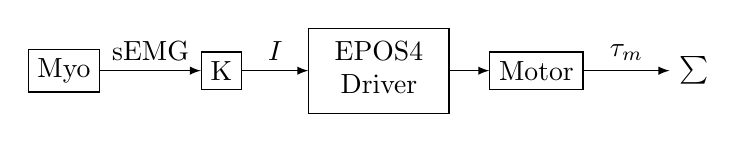
\begin{tikzpicture}[auto, node distance=2cm,>=latex]
        \tikzstyle{block} = [draw, rectangle]
        
        \node [block, draw] (input) at (0,0) {Myo};
        \node [block, right of=input, node distance=2cm] (gain) {K};
        \node [block, right of=gain, node distance=2cm] (driver) {
          \begin{tabular}{c}
            EPOS4\\ 
            Driver
          \end{tabular}
        };
        \node [block, right of=driver, node distance=2cm] (motor) {Motor};
        \node [right of=motor] (sys) {$\sum$};

        \draw [->] (input) -- node[above] {sEMG} (gain);
        \draw [->] (gain) -- node[above] {$I$} (driver);
        \draw [->] (driver) -- (motor);
        \draw [->] (motor) -- node[above] {$\tau_m$} (sys);
    \end{tikzpicture}
    \caption{
      Simplified Control Diagram - $K$ is an arbitrary gain 
    }
    \label{fig:simplified_control_diagram}
\end{figure}
\end{frame}

\section{Possible Improvements}
\begin{frame}{Possible Improvements}
Torque estimation:
\begin{itemize}
\item Using different input parameters for the NN models
\item User load estimation (e.g. with an extended state observer)
\item Adding a Model Reference Adaptive Controller
\item Improving the estimation of the K gain
\end{itemize}
Control strategy:
\begin{itemize}
\item Control position instead of current
\item Improving the quality of the training data
\item Modifying the NN model architecture 
\item Smoothing the NN output
\end{itemize}
\end{frame}

\section{Conclusion}
\begin{frame}{Conclusion}
\end{frame}

\end{document}
